\chapter{Experiment and Evaluation - System Performance}
\section{Goals}
This experiment is just a proof of concept to show that Graphy's data models for tags and relationships can be exchanged and synchronized between mobile clients like other Contacts application with similar performance. The goals of the experiment are as follows:

\begin{itemize}
    \item Clients can push contact data to backend server.
    \item Clients can pull contact data from backend server.
    \item Clients can synchronize their contact data with each others (through the help of the backend server).
    \item Clients can resolve contact data conflicts between each others (through the help of the backend server).
\end{itemize}

\section{Experimental Setups}
abc

\begin{figure}[!h]
\begin{centering}
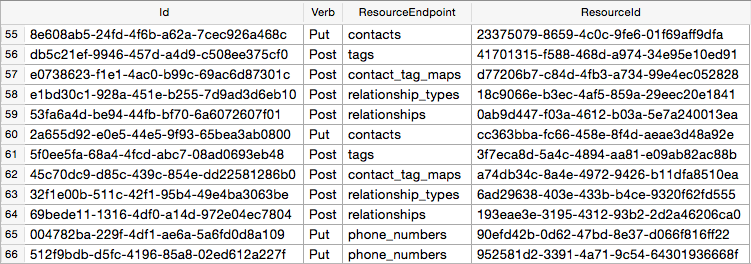
\includegraphics[scale=0.63]{pics/sync_queue.png}
\caption{Sync Queue Table}\label{fg:sync_queue}
\end{centering}
\end{figure}

\section{Scenarios and Results}
abc

\begin{table}[!ht]
\centering
\caption{abc}\label{tb:abc}
\begin{tabular}{ | c | c | }
\hline
	Creation/Modification & Retrieval \\ \hline
	9.5877 & 4.0301 \\ \hline
	9.7471 & 4.5846 \\ \hline
	9.8455 & 5.0286\\ \hline
	9.4878 & 4.2998\\ \hline
	9.5682 & 4.6329\\ \hline
	9.6295& 4.9852\\ \hline
	10.1144 & 5.0014\\ \hline
	9.5907 & 4.2031\\ \hline
	10.4971 & 4.8837\\ \hline
	9.7939& 4.9016\\ \hline
	\  & \  \\ \hline
        \textbf{9.7861}& \textbf{4.6551}\\ \hline
\end{tabular}
\end{table}

\begin{figure}[!h]
\begin{centering}
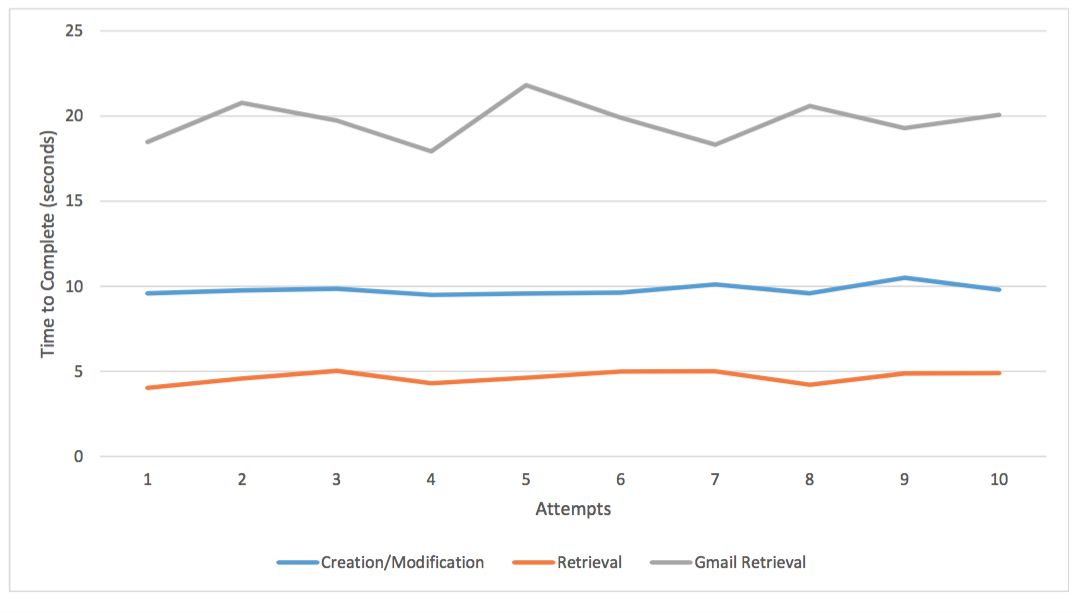
\includegraphics[scale=0.4]{pics/system_performance.png}
\caption{abc}\label{fg:system_performance}
\end{centering}
\end{figure}

\section{Conclusion}
